% by Mirella M. Moro; version: January/18/2012 @ 04:16pm
% -- 01/18/2012: more discussion on SBBD + JIDM; overall revision
% -- 09/03/2010: bib file with names for proceedings and journals; cls with shrinked {received}
% -- 08/27/2010: appendix, table example, more explanation within comments, editors' data

\documentclass[jidm,a4paper]{jidm} % NOTE: JIDM is published on A4 paper
\usepackage{graphicx,url}  % for using figures and url format
\usepackage[T1]{fontenc}   % avoids warnings such as "LaTeX Font Warning: Font shape 'OMS/cmtt/m/n' undefined"

%\usepackage{cite} % NOTE: do **not** include this package because it conflicts with jidm.bst

% Standard definitions
\newtheorem{theorem}{Theorem}[section]
\newtheorem{conjecture}[theorem]{Conjecture}
\newtheorem{corollary}[theorem]{Corollary}
\newtheorem{proposition}[theorem]{Proposition}
\newtheorem{lemma}[theorem]{Lemma}
\newdef{definition}[theorem]{Definition}
\newdef{remark}[theorem]{Remark}

% New environment definition
\newenvironment{latexcode}
{\ttfamily\vspace{0.1in}\setlength{\parindent}{18pt}}
{\vspace{0.1in}}

% ALL FIELDS UNTIL BEGIN{document} ARE MANDATORY

% The following data (volume, number and page) are given by the editors prior to publishing your article
\jidmVolume{5}
\jidmNumber{1}
\jidmYear{14}
\jidmMonth{June}
\setcounter{page}{1}


% Includes headers with simplified name of the authors and article title
\markboth{M.N. Amorim, R.M.C. Segundo, C.A.S. Santos}
{JIDM - Journal of Information and Data Management}
%  -> \markboth{}{}
%         takes 2 arguments
%         ex: \markboth{M. M. Moro}{Any article title}


% Title of the article
\title{LiveSync: a Tool for Real Time Video Streaming Synchronization from Independent Sources}


% List of authors
%IF THERE ARE TWO or more institutions, please use:
%\author{Name of Author1\inst{1}, Name of Author2\inst{2}, Name of Author3\inst{2}}
\author{Marcello N. de Amorim\inst{1}, Ricardo M. C. Segundo\inst{2}, Celso A. S. Santos\inst{3}}


%Affiliation and email
\institute{Universidade Federal do Espirito Santo, Brazil  \\ \email{novaes@inf.ufes.br , rmcs87@gmail.com , saibel@inf.ufes.br}
% IF THERE IS ANOTHER INSTITUTION:
%\and Name_of_the_second_institution \\
%\email{address@whatever.com}
}


% Article abstract - it should be from 100 to 300 words
\begin{abstract}
This work presents a method that allows users to synchronize live video streams from multiple sources, such as YouTube and several other video streaming sources, as well as a web application for ease its use. The proposed method for pursuing multi-camera video streaming synchronization is based on a crowdsourcing approach, using the human processing-power of a crowd of contributors to synchronize videos, requiring each user to find only one synchronization point for a single couple of video streams. Additional synchronization is inferred from the processed contributions, using transitivity properties and an appropriate structure for this inference, the Dynamic Alignment List.
\end{abstract}


% ACM Computing Classification System categories
\category{H.4.4.3}{Information Systems Applications}{Crowdsourcing} 
\category{H.3.2.7}{Human-Centered Computing}{Synchronous editors}

% Categories and Descriptors are available at the 1998 ACM Computing Classification System
% http://www.acm.org/about/class/1998/
%  -> \category{}{}{}
%         takes 3 arguments for the Computing Reviews Classification Scheme.
%         ex: \category{D.3.3}{Programming Languages}{Language Constructs and Features}
%                   [data types and structures]
%                   the last argument, in square brackets, is optional.

% Article keywords
\keywords{live video, synchronization, crowdsourcing}
%  -> \keywords{} (in alphabetical order \keywords{document processing, sequences,
%                      string searching, subsequences, substrings})


% THE ARTICLE BEGINS
\begin{document}

% This is optional:
\begin{bottomstuff}
%The authors would like to thank the "Fundação de Amparo à Pesquisa e Inovação do Espírito Santo" (FAPES) and "Coordenação de Aperfeiçoamento de Pessoal de Nível Superior" (CAPES) for financial support.
\end{bottomstuff}

\maketitle

\section{Introduction}

User generated videos (UGV) live streaming continuously grows in number end relevance boosted by platforms such as Facebook, Youtube and Vimeo. Into this scenario is relevant find out methods capable to synchronize them. 

Automatic methods are widely used to reach video synchronization. Although, they generally demand vast example databases as well controlled conditions, standardized structure and marks to work properly \cite{wang2014videosnapping}. These methods usually present good results synchronizing well-structured video productions, professional coverage for sport events and other modalities of planed videos. However, they tends to face challenges attempting to synchronize heterogenous videos in situations where have to deal with wide baselines, camera motion, dynamic backgrounds and occlusion \cite{schweiger2013fully}.

UGV are produced over the user's point of view, so different users covering a same event tends to result in heterogeneous video streams, in different angles, qualities, audio content, and other characteristics that make automatic methods unappropriated to synchronize these sources.

To achieve synchronization for UGV live streamings from different sources,  this work introduces LiveSync, a method that explore the human ability of associate  heterogeneous videos. LiveSync is based on the Human Computation paragidm \cite{VonAhn:2005:HC:1168246}, using human intelligence to execute tasks usually hard to machines but easy to ordinary people using its senses (vision and hearing). Additionally, human computation can improve performance by division of labor because it helps to define tasks that can be executed in parallel \cite{Rohwer:2010:NHC:1837885.1837897}. This characteristic is potentialized in LiveSync by adopting a crowdsourcing approach, to use efficiently the processing power of a crowd of collaborators, collecting their contributions in parallel \cite{howe2006rise} . 

Crowndourcing is an approach in which a problem is divided in tasks, and the execution of these tasks is delegated to the crowd composed by individuals engaged in the solution process. The partial result delivered by each contribution are registered, and a final outcome is generated by processing them. A very popular crowdsourcing strategy consists in to distribute tasks that can be completed easily and quickly \cite{Difallah:2015:DMC:2736277.2741685}.

The application scenario for LiveSync contains a set of UGV live streams from different sources, that must be synchronized. These synchronization issues are related to time delays between videos streamed from different sources. The occurrence of time delay between a pair of videos is manifested as misalignment, in other words, there is a time difference between scenes that should be displayed at the same time.  In this work the time delay between a pair of videos if refereed as $\Delta{time}$.

In the proposed method is created a list with all possible pairs of video streams, and each collaborator is asked to provide a synchronization point for one pair.  The delay between each pair of streams is determined by processing the contributions, and the streams are aligned based on these delays, making possible to align them in a synchronized presentation.

This paper extends the previous work "LiveSync: a tool for Real Time Video Streaming Synchronization from Independent Sources" \cite{delivesync} presented in the XXII Brazilian Symposium on Multimedia and Web Systems (WebMedia 2016) where it was honoured with the Best Paper Award at XVI Workshop of Tools and Applications (WFA).

This remain of this work is organized as follows: section 2 describes method LiveSync, section 3 details LiveSync Tool, section 4 presents an study case to evaluate the proposed method. Finally, section 5 concludes with some remarks about this work and further research.   




\subsection{Dinamic Aligment List}

The Dynamic Alignment List (DAL) is an abstract datatype designed to organize the relations (relational couplers) between videos as well to provide the features required to store and process the relations. Each relation stored into a DAL instance corresponds to a relational coupler related with a pair of video streams and the $\Delta{time}$ between them.


The start model for the storage structure inside the DAL was a relational matrix MxM which can represent all possible relations between M videos, each position representing the $\Delta{time}$ between the initial point of a pair of videos. This matrix was reduced to a upper triangular matrix because $\forall{i,j} < M , \Delta_{i,j}$ = $- \Delta_{j,i}$ and the main diagonal was eliminated because $\Delta_{i,j}$ is always equal to zero. The $\Delta{time}$ for each couple of videos is calculated for $\Delta{i,j} = start(j) - start(i)$ where $start(X)$ returns the offset of video X from the start of the event's timeline.

These values are used to synchronize the M videos. If $\Delta{i,j} > 0$ the video $i$ starts before the video $j$, if $\Delta{i,j} < 0$ the video $i$ starts after the video $j$, and when $\Delta{i,j} = 0$ both videos start at the same time. The values are represented in milliseconds, so $\Delta{i,j} = 30$ means the video $j$ should starts 30 ms after the video $i$ starts in order to achieve their synchronization. Additionally, in cases which is impossible to determine a relation between a pair of videos, the value registered is $I$ that means impossible.

Into a collaborative scenario where users can contribute providing a $\Delta{i,j}$ for a pair of videos $(i,j)$, it is important to store all contributions, because the $\Delta{time}$ value should be calculated considering the contributions collected for that pair. In that approach the formula $\Delta{i,j} = start(j) - start(i)$  is used to calculate the $\Delta{time}$ for each contribution, and the value stored in DAL is determined processing all contributions for each pair. Moreover, the number of contributions for each pair can grow while the contribution process is active, and current $\Delta{time}$ of a pair can change while contributions are incoming.

In order to represent this model it was needed to define a structure more sophisticated then a matrix. This structure preserves the relational characteristics of a upper triangular matrix without the main diagonal, with an additional dimension related to the contributions for each relation between video pairs. However, it is implemented as a hash table, using linked lists hierarchically organized in three levels. 

\begin{itemize}

\item Level 1 - The first level is a list of video structures. Each structure has a unique identification label for a correspondent video. 

\item Level 2 - Each video structure points to a second level linked list composed by all possible relations that include its video, considering the relations in a upper triangular matrix without the main diagonal.  Thus, each node in a second level linked list corresponds to a relation between it's video represented in its root and another video.

\item Level 3 - Each relation in a level 2 list points to a third level list, in which each node represent a contribution for that relation.

\end{itemize}

Figure~\ref{dal} exemplify a data structure into a DAL with 5 videos. The videos, labeled as $A, B, C, D$  and $E$, are in the fist level linked list. Each video points to a second level list, it is possible to observe in Figure~\ref{dal}  that each second level linked list have only the relations that would exist in a single line of a upper triangular matrix without the main diagonal. Moreover, in Figure~\ref{dal} each relation, that is an element of second level list, points to a cloud that represents a third level list with all contributions for that relation.

\begin{figure}
	\centering
	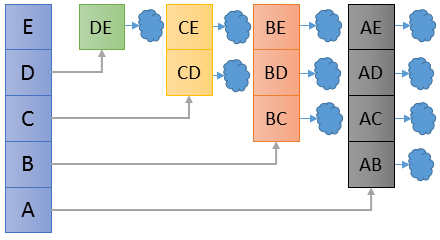
\includegraphics[scale=0.8]{figures/dal}
	\caption{DAL with 5 Videos (A,B,C,D,E)}
	\label{dal}
\end{figure}

A completed DAL can provide all information needed to achieve synchronization for videos registered on it, although it is more than a data structure. DAL is an abstract datatype that provides the data structure plus a set of features that allows access, manage and process the information inside it, such as the function \textit{Infer Synchronization}. 

\textit{Infer Synchronization} can obtain additional relations by executing an inference algorithm over the current relations. This algorithm checks if is possible to find an indirect path between two videos by transitivity. For example, considering the videos $A, B$ and $C$, if the relations $AB$ and $BC$ are known, by transitivity is possible to infer the relation $AC$. This feature can reduce the number of contributions required to complete a DAL. 





\section{LiveSync}
Live synchronization includes the scenario where a viewer has access to an event that is live streamed by more than one Content Provider. These content providers are independent, so their videos do not have initial resources that allow their automatic synchronization to viewers, requiring a video analysis to generate synchronization points (Couplers). This synchronization fits as a problem that can be solved by using the power of the crowd. This occurs because videos are generated independently, without synchronization points and without previous description of what is about to be shown in screen, neither how can it be correlated to other videos. This way, human perception is used in real time to generate unknown synchronization points. 

As example for this scenario, we can take a public manifestation. In the event, multiple people can take their cell phones and start streaming the event. In their house, other people can watch the videos. However, the multiple videos from different sources will be asynchronous. We need a way to synchronize these UGV. We use the crowd to achieve it. To this objective we group all videos in a MashUp application that connects to a Coupler Server that contains all synchronization data. Both synchronizing and playing the videos are made using this mashup, that can receive videos from multiple sources.






%%%%%%%%%%%%%%%%%%% ACM %%%%%%%%%%%%%%

Live synchronization includes the scenario where a viewer has access to an event that is live streamed by more than one Content Provider. These content providers are independent, so their videos do not have initial resources that allow their automatic synchronization to viewers, requiring a video analysis to generate synchronization points (Couplers).

As example for this scenario, we can take a public manifestation. In the event, multiple people can take their cell phones and start streaming the event. In their house, other people can watch the videos. However, the multiple videos from different sources will be asynchronous. We need a way to synchronize these UGVs. We use the crowd to achieve it. To this objective we group all videos in a mashup application that connects to a Coupler Server that contains all synchronization data. Both synchronizing and playing the videos are made using this mashup, that can receive videos from multiple sources.

In a live presentation, it is assumed that content must be consumed right after its generation. It is of extreme importance that the synchronization method can be performed in playback time, to allow the integration of live content. However, not all viewers are required to be part of the crowd to achieve synchronization. If a synchronization made by a single member of the crowd is accepted as accurate, it can be transferred to the remaining viewers, this way each one will have his content locally synchronized.

One way of live synchronization can work is as follows: a person selects and synchronizes two videos with the help of a manipulation tool. This becomes a candidate synchronization point. Several people can do the same, and the results can be based on multiple synchronizations. Having these synchronization points defined, synchronization information can be sent to other viewers interested in watching those videos. As simple example, take two independent sources that are transmitting an event. A mashup system allows the user to watch both videos at the same time is his device. However the videos are asynchronous and the user notices that. He then access the option to synchronize the videos. After he achieve a synchronous result, implicitly his contribution is sent to a server that will feed other users that choose to watch the same videos with the synchronization specification. If the user thinks the content is not synchronised yet, he can synchronize it himself and send another contribution. This tool was implemented and is presented on section~\ref{livesync}.







\subsection{Method}

Video live streams are associated to real-time delivery, so it is an important characteristic of LiveSync allow users to play the streams while attempt to find synchronization points between then. In this way, users can consume this live content while performing their contribution tasks.

When performing a synchronizing task, the user don't need analyses entire videos seeking for synchronization point. An user can simply use the buttons Play and Pause on the video player until both videos are playing synchronously. Once the user archived a local synchronism to a pair of videos, the application measure the delay between them and registers it as a $\Delta{time}$ contribution. All contributions are registered, and used as input to calculate the delay between each pair of videos that will likely satisfy users.

As soon as a pair of videos are synchronized, the application registers this synchronization and align the videos in a visualization interface with the other synchronized videos. So, anyone may access this view and watch the synchronized videos in an aligned view.


\section{LiveSync Tool}

\subsection{Main Functionalities}
The main functionalities provided by the LiveSync Tool are:

\begin{description}
	\item[Synchronized Live Video Player -]	the tool permits users to watch multiple videos synchronized. He selects from a list of sources the videos he wish to watch and them they are synchronized using information provided by other users.
	
	\item[Video Synchronization -] If a pair of videos does not have any information about their synchronization, users are invited to contribute and synchronize the videos.
	
	%\item[Infer Synchronization -] Additional relations can be obtained executing an inference algorithm over the already converged relations. This algorithm check if is possible to find a indirect path between two videos by transitivity. For example, considering the videos $A, B$ and $C$, if the relations $AB$ and $BC$ are known, by transitivity is possible to infer the relation $AC$.
		
	\item[Video Aggregation -]	Although the focus of the LiveSync Tool is UGV live streams synchronization, it must to allow users to add new stream sources to the application. He only needs to set the video source, and the video will be added to the DAL and list of videos. However, videos added are not filtered, this means that the user can add any video to the application, even ones that contains none relation with the other videos. In future versions will be added an functionality to users mark which video as not related, and then remove them.
	
	\item[Multiple Platforms Support -] One key-point on this tool is to use other platforms as video sources. The videos presented to users, and synchronize by them, are provided by external live video stream platforms. To be compatible with LiveSync Tool are required two requisites:
	\begin{enumerate}
		\item Remote Player: the platform must allows embeddability into player on third pages, allowing us to control the player with its basic functionalities such as: play, pause and stop;
		\item Uptime Support: a second and fundamental requisite is an API that allows video uptime retrievement. Video uptime is the time since the beginning of the video that is presented on the video player. This is fundamental to create and replicate the temporal couplers used to play the synchronized video streams.
	\end{enumerate}
	
	\item[Serverless Architecture -] Serverless architectures refer to applications that significantly depend on third-party services and putting much of the application behavior and logic on the front end. Such architectures remove the need for the traditional server system sitting behind an application \cite{RobertServerless}.
	
	\item[Multiplatform -] LiveSync is a Web Based application designed and developed in compatibility with HTML5 standard to its front-end (Mash-up Player) component. It allows this application to be executed on multiple browsers, operational systems and devices.
	
	\item[Active vs Passive Contributions -] Currently  exist two versions for LiveSync Tool that only differ in what pair of videos should be synchronized by each user. The active version allow users to navigate freely through the videos, synchronizing them when they wish to. The Passive Contribution version uses an automatic algorithm to ask users which pair of videos they should synchronize.

	
\end{description}

\subsection{Architecture}
The LiveSync tool has three main components (Figure~\ref{livesync}): the Content Providers (Video Sources), the Coupler and the Mashup Player.

\begin{figure}[h]
	\centerline{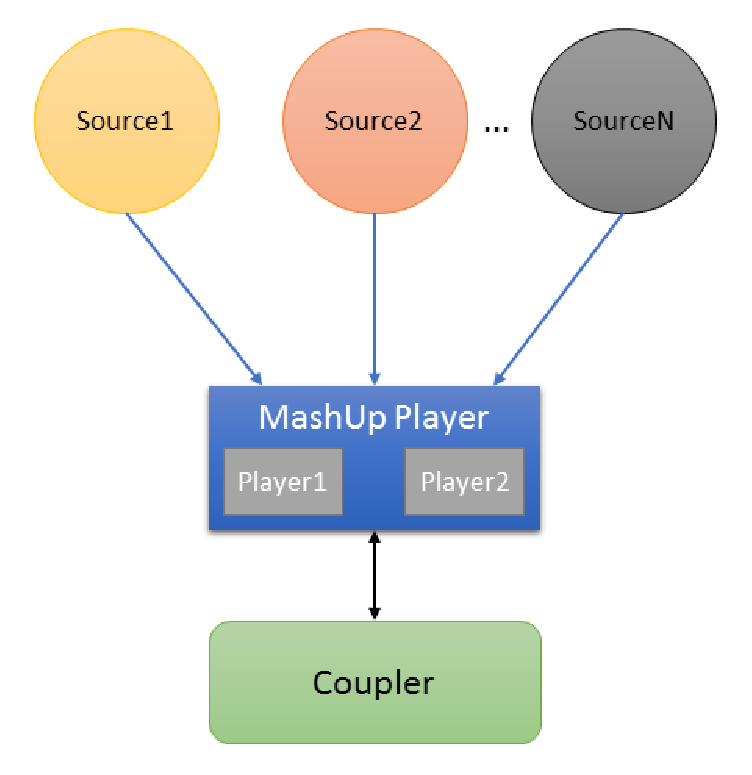
\includegraphics[scale=0.6] {figures/architecture}}
	\caption{Modelo simplificado do live-sync}
	\label{livesync}
\end{figure}

\subsubsection{Content Providers}
Content Providers are third-parties videos streamers platforms, such as YouTube Live, LiveStream, TwitCast, Twitch and Ustream. LiveSync Tool supports different platforms as video sources, maximizing the number of videos streams that can be related to an event.

There are two requirements that a Content Provider must attend to be compatible with LiveSync: Remote Player and Uptime Support.

As each flow platform uses its own protocols, the embedded players are required for aggregation in the mash-up application. These players must provide buttons to play, pause and stop actions.

Uptime Support, is necessary to find the temporal couplers to video streams. Uptime is the time passed since the beginning of the live stream until the video part being presented in the player at the moment of the call.


\subsubsection{Coupler}
The Coupler is responsible for storage, distribution and calculation of synchronization points among video streams from the Content Providers.

An instance of coupler is composed of a DAL instance and Log files. This goes in direction of the Serverless Architecture. We wanted an architecture that needed low resources (another justification for using third party stream services) and easy deployment. All that is necessary do execute the coupler is a NODE.JS (https://nodejs.org/en/) server instance. This is possible because the coupler is fully developed in JavaScript and compatible with the HTML5 standards. To deploy the coupler, we use a Backend as a Service or ”BaaS” platform, more specifically we use the Heroku (www.heroku.com) one, that permits free use of NODE.JS instances.

It stores synchronization information only during the duration of the event, so its stance is finished with the end of the videos and all data is lost. In the current scope, the sync info is only necessary during the event, after it, there is no need to store the information. For reasons of testing and using the filmed videos from YouTube we create log files that contains all contributions made by the crowd. If it is important to maintain all contributions and data for post analyses and further use, unstable version of the LiveSync is being configured to use a fully transactional database. We use a fully transactional database because we want to maintain track of all contributions made by the crowd, an important aspect for crowdsourcing support and that is also supported by the DAL.

Other aspect of the coupler is that it is responsible for the distribution of synchronization couplers. When a user chooses two videos, a message is sent from the mash-up to the coupler, containing the required relation. The coupler then answer with the required information. If the relations is unknown, it answer soliciting the user to synchronize and contribute with those two videos.

The last function of the coupler, is to calculate the synchronization points among Videos. Each relation ($\Delta_{A,B}$) may contain several contributions, then it is necessary to calculate a value to that relation based on the contributions. In the current version we calculate a Geometric Mean of the contributions to find an ideal value. This however may not be the best value, because the more accurate the sync is, the better the results are, so older contributions must have a lighter weight, something that does not happen in current version. The other calculation made by the Coupler, is to infer unknown relations based on the afore mentioned transitive relation.

The communication  between coupler and mash-up is made through Websocket communication. The mash-up creates a WebSocket channel with the Coupler, and requests the sync information or sends contributions from the crowd. A simple protocol is used in JSON messages: {act:value, data:object}. The act field contains the action to be made and the data contains an object to complement the action. As example we have an act to send a new contribution ("contribution") that is complemented with a new relation that contains the videos involved, the value and an id to that contribution.



\subsubsection{MashUp Player}

Mash-ups are applications generated by combining content, presentation or other applications functionalities from disparate sources. They aim to combine these sources to create useful new applications or services (the offer and consumption of data between two devices) to users. The LiveSync Tool combines videos from different sources with synchronization information from the Coupler Service to reproduce a synchronous presentation for these videos. The Mash-up Player is used to both presenting video synchronously and collecting the synchronization values. 

At the top of the interface all information necessary to the user as may be observed on Figure~\ref{menu_add_view}. Fallowing the orientations on the screen an user can select which videos want to watch, add a new videos, as well start the synchronization process for videos that he believes are not synchronized. 

\begin{figure}[h]
	\centerline{
\includegraphics[scale=0.3] {figures/menu_add_view}}
	\caption{Action menu at the top of interface}
	\label{menu_add_view}
\end{figure}

When an user adds a video, an input text is shown to him, so he can add the video URI (WebSocket) or video ID YouTube). The page reloads and the new video is listed in the video list for everyone that connects to the application. Also, when the video is added by the user, an message is sent to the Coupler Service, containing the action to add a new video to the DAL, and the specification of it, such as label and URI.

When just playing two selected videos from the videos list, each for video player is created an instance that is compatible with that source (YouTube or WebSocket). Moreover, it is invisible to users where the video is coming from.

The last functionality of the mash-up is to synchronize the videos. When an user chooses to synchronizing a pair of videos, the mash-up display is reconfigured and the application enter in synchronization mode. LiveSync Tool uses a Play ’n Pause approach to synchronize the videos. Figure~\ref{live_tvs} represents the interface of the mash-up during a test: two cameras live streaming (content providers) a simulated television event to our mash-up application. Once the user decided the videos are synchronized he clicks on the done button, so his contribution committed to the Coupler Service that stores it into the DAL for further processing of the relation.

\begin{figure}[h!]
	\centerline{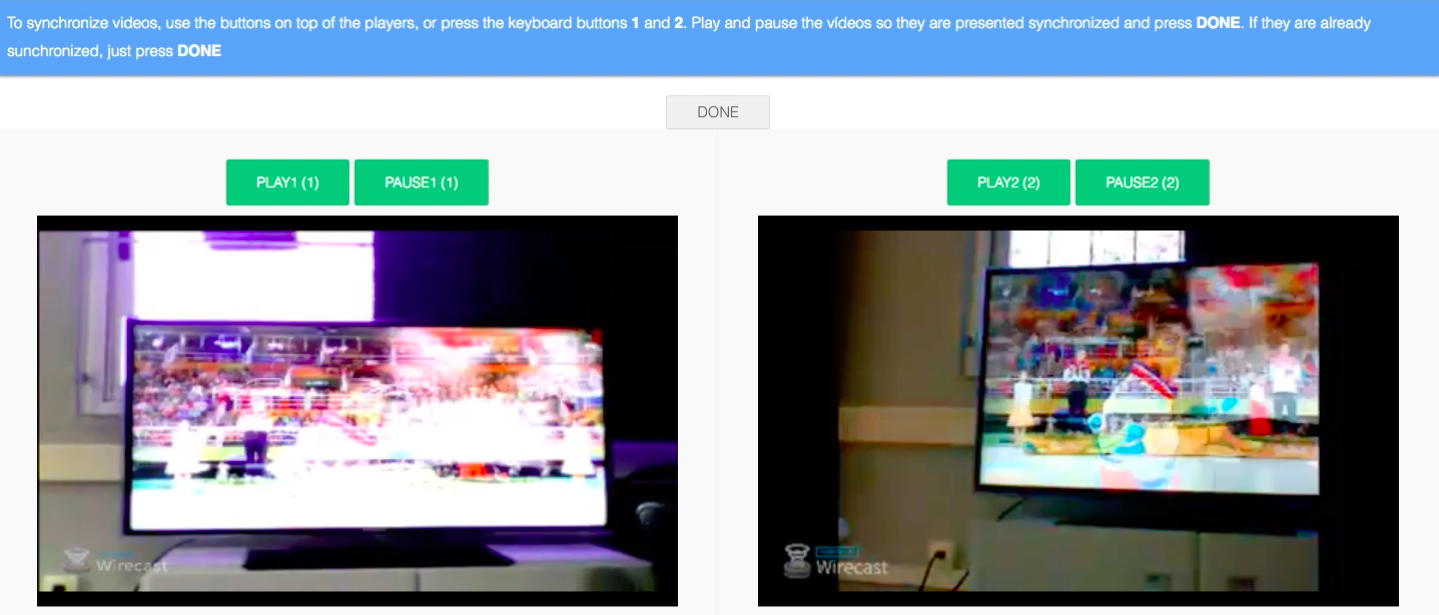
\includegraphics[scale=0.3] {figures/screen}}
	\caption{Live Streams from Olympic Games Synchronized through two different cameras}
	\label{live_tvs}
\end{figure}




\section{Experiment - XXXXXXXXXX}
\textbf{TO DO}

\section{Final Remarks}
%(5) Conclusão, limitações, trabalhos futuros.

LiveSync is a method that aims achieve UGV live streams synchronization. The focus of this method is cover the scenarios where automatic techniques facing problems to work properly. The approach adopted in LiveSync is to use do work-power of a crowd of contributors to executing small tasks generally easy for humans but hard to machines, registering these contributions and using it to determine the synchronization points between videos. This approach assume that human perception is better than automatic techniques to synchronize heterogenous and non standardized UGV.

The LiveSync Tool is a Web implementation for LiveSync that allows users contribute in UGV live streaming synchronization processes, as well to watch synchronized UGV live streams from multiple sources. However, this tool presents some limitations that shall in the futures be suppressed, such as the number of events that we can follow. Now, each instance of Coupler and mash-ups can handle only one event, in other words, we can not cover two independent live events at the same time with one instance, for that porpoise we need more than on instance of each service. Also, new stream services must be added to increase our compatibilities.

All code for LiveSync Tool may be freely downloaded from Github \url{https://github.com/rmcs87/liveSync}.


\bibliographystyle{jidm}
\bibliography{jidmb}

\end{document}
